\documentclass[aspectratio=43, 10pt]{beamer}
\usepackage{tutorialSlide}
\usepackage{graphicx}               % Necessary to use \scalebox
\usepackage[absolute,overlay]{textpos}
\usepackage{enumitem}
\usepackage[dvipsnames]{xcolor}
\usepackage[inkscapelatex=True]{svg}
\usepackage{svg}
\usepackage{adjustbox} % 用于缩放图片
\usepackage{fontawesome}
\usepackage{MnSymbol,wasysym}


\newcommand{\curl}{{\textbf{curl}}}


\mode<presentation> {
\usetheme{AnnArbor}
\usecolortheme{dolphin}

\setbeamercolor{alerted text}{fg=red}
% Change color scheme for blocks
\setbeamercolor*{block title example}{fg = ao(english), bg= antiquewhite}
\setbeamercolor*{block title}{fg = pigment, bg= blue!5}
\setbeamercolor*{block title alerted}{fg = red, bg= red!5}
}

\makeatletter
\newcommand\mysphere{%
  \parbox[t]{8pt}{\raisebox{0.2pt}{\beamer@usesphere{item projected}{bigsphere}}}}
\makeatother




%***************************************************************************
%***************************************************************************
\begin{document}
\title[Safe RL]{Constrained Reinforcement Learning with \\ Cumulative or Instantaneous Constraints}
\subtitle{}
\author[ Speaker: William Weijia Zheng ]{William Weijia Zheng}

\institute[IE@CUHK] 
{
\textit{Department of Information Engineering} \\ % Your institution for the title page
\textit{The Chinese University of Hong Kong} \\
\medskip
wjzheng@link.cuhk.edu.hk % Your email address
}
\date{January 09, 2026}

\setcounter{framenumber}{-1}
\frame{\titlepage}
%***************************************************************************
%***************************************************************************




\begin{frame}
\frametitle{Overview} % Table of contents slide, comment this block out to remove it
\tableofcontents % Throughout your presentation, if you choose to use \section{} and \subsection{} commands, these will automatically be printed on this slide as an overview of your presentation
\end{frame}



\AtBeginSection[]
  {
     \begin{frame}<beamer>
     \frametitle{Overview}
     \tableofcontents[currentsection]
     \end{frame}
  }
  

\section{Problem Statements of (PC) and (PI)}    
    \begin{frame}{Cumulatively Constrained RL}

        Let $t \in \mathbb{N} \cup \{0\}$ denote the time instant and $S \subset \mathbb{R}^n$, $A \subset \mathbb{R}^d$ denote states and actions of an agent described by a Markovian dynamical system with transition density $p: s_{t+1} \sim p(\cdot | s_t,a_t)$. The agent chooses actions sequentially based on a policy $\pi \in \mathcal{P}(S)$, space of probability measures.  

        \vspace{0.2cm}

        The goal of (cumulatively) constrained RL (CRL) is to find a policy $\pi^* \in \mathcal{P}(S)$ that meets these objectives by solving the following problem: 
        \begin{align}
            \tag{PC}
            \max_{\pi} &~~ V_0(\pi) \triangleq \mathbb{E}_{s,\pi} \left[ \sum_{t=0}^{\infty} \gamma^t r_0(s_t, \pi(s_t)) \right]  \\
            \text{subject to } & V_i(\pi) \triangleq \mathbb{E}_{s,\pi} \left[\sum_{t=0}^{\infty} \gamma^t r_i(s_t, \pi(s_t))  \right] \geq c_i, i \in \{1,2,...,m\}. \notag
        \end{align}

        \vspace{0.2cm}
        If one removes the constraints, (PC) degenerates back to "usual" RL formulation, which can be tackled by some standard RL algorithms. 

        \textcolor{red}{We'll soon spend some time to see that (PC) can be "solved" by primal-dual methods.}
        
    \end{frame}

    \begin{frame}[t]{Instantaneously Constrained RL}
        The goal of instantaneously constrained RL is to find a policy $\pi^* \in \mathcal{P}(S)$ that meets these objectives by solving the following problem: 
            \begin{align}
                \tag{PI}
                \max_{\pi} &~~ V_0(\pi) \triangleq \mathbb{E}_{s,\pi} \left[ \sum_{t=0}^{\infty} \gamma^t r_0(s_t, \pi(s_t)) \right]  \\
                \text{subject to } & ~\mathbb{E}_{\pi} \left[  r_i(s_t, \pi(s_t))  \right] \geq 0,~~  \forall t \in \{0,1,...\}, i \in \{1,2,...,m\}. \notag
            \end{align}

        Note that the constraints are applied for \textbf{every time instant} $t$, rather than a long-term weighted sum. 

        We remark here that an optimal policy feasible for (PI) could be a conservative but feasible solution for (1). 
        
        If the policy $\pi$ is deterministic, then the constraints will become: 
        \begin{equation}
            r_i(s_t, \pi(s_t)) \geq 0, ~~\forall t \in \{0,1,...\}, \forall i \in \{1,2,...,m\}. 
        \end{equation}

        \textcolor{red}{We will see why (PI) cannot be easily solved under the framework of (PC).}

        \textcolor{teal}{I want to make the slides self-contained. So I include some proofs. I tried to make them as simple as they should be.}

    \end{frame}    

\section{Strong duality holds for (PC)}
    \begin{frame}[t]{Strong duality proof p1: an important lemma} 
    \vspace{-0.4cm}
    \begin{columns}
        \begin{column}{0.52\textwidth}
            \begin{lemma}[no need for $V_0(\cdot),...$ convex.]
                If Slater's condition holds for (PC) and its perturbation function $P(\xi)$ is concave, then strong duality holds for (PC). 
            \end{lemma}
        \end{column}
        \begin{column}{0.4\textwidth}
            \begin{align*}
                  & P(\xi) \triangleq \max_{\pi} \  V_0(\pi) \\
                  \text{s.t. } & V_i(\pi) \geq c_i + \xi_i, \ i = 1,\dots,m.
              \end{align*}
        \end{column}
    \end{columns}
    \begin{proof}
        First, note that $P(\boldsymbol{0})=P^*$. Our goal is $P^*=D^*$. 
        Weak duality always holds: $P^* \leq D^* \triangleq \min_{\lambda\geq 0}d(\lambda)= \min_{\lambda\geq 0} \max_\pi V_0(\pi) + \sum_{i=1}^m \lambda_i (V_i(\pi)-c_i)$. 
        
        Slater's condition implies that $\boldsymbol{0} \in$ interior of domain of pert. problem $P(\cdot)$.  
        As $P(\xi)$ is concave in $\xi$, $\exists \lambda \in \mathbb{R}^m$ s.t. $\forall \xi$, $P(\xi)\leq P( \boldsymbol{0}) + \lambda^T \xi$. (superdifferential)

        \pause 
        Further note that those $\lambda \leq 0$. Otherwise, pick $\lambda_j >0$ and $\xi_j <0, ~(\xi_i=0, \forall i\neq j)$, we have the following contradiction: 
        $$P(\boldsymbol{0}) \leq P(\xi) \leq P( \boldsymbol{0}) + \lambda^T \xi < P(\boldsymbol{0}).$$
        
        Then, $ \mu = -\lambda \geq 0$, 
        $P^* \geq \sup_{\xi} P(\xi) + \mu^T \xi  = \sup_{\pi, \xi: V(\pi)\geq c+\xi} V_0(\pi)+ \mu^T \xi = \sup_{\pi} V_0(\pi)+\mu^T (V(\pi)-c) = d(\mu).$ 
        Thus $D^* = \min_{\mu'}d(\mu')\leq d(\mu) \leq P^*. $
    \end{proof}
    
    \end{frame}

    \begin{frame}[t]{Strong duality proof p2: $P(\xi)$ is concave} 

        \vspace{-0.3cm}
        \begin{itemize}[leftmargin=*, itemsep=1em]

        \item Transform (via some tedious but standard algebra) the perturbed problem into a \textbf{linear program} over \textbf{occupation measures} $\rho(s,a)\triangleq (1-\gamma) \sum_{t=0}^\infty \gamma^t p_{\pi}^t (s,a)$:
              \begin{align*}
                  P(\xi) =& \max_{\pi \in \mathcal{P}(S)} V_0(\pi)= \max_{\rho \in \mathcal{R}} \ \frac{1}{1-\gamma} \int r_0(s,a) \rho(s,a) \, dsda \\
                  \text{s.t. } & V_i(\pi) = \frac{1}{1-\gamma} \int r_i(s,a) \rho(s,a) \, dsda \geq c_i + \xi_i.
              \end{align*}
              where $\mathcal{R}$ is the set of all valid $\rho(\cdot, \cdot)$'s, the discounted state-action occupancies. A crucial property (from Borkar '88) is: $\mathcal{R}$ is a \textcolor{teal}{convex and compact} set. 

        \pause 
        
        \item \textbf{Concavity follows}: For two perturbations $\xi^1, \xi^2$, let $\rho_1, \rho_2$ be their underlying optimal occupancies. For any $\mu \in (0,1)$, the convex combination $\rho_{\mu} = \mu \rho_1 + (1-\mu)\rho_2$ exists (via \textcolor{teal}{convexity} mentioned above, denote its policy as $\pi_\mu$), and is feasible for $\mu \xi^1 + (1-\mu)\xi^2$ because constraints are linear in $\rho$. Thus,
              \[
                  P(\mu \xi^1 + (1-\mu)\xi^2) \geq V_0(\pi_\mu) = \mu V_0(\pi_1) + (1-\mu)V_0(\pi_2) = \mu P(\xi^1) + (1-\mu) P(\xi^2).
              \]
              The above inequality's head and tail match the definition of concavity.
    \end{itemize}
    \end{frame}

    \begin{frame}[t]{Parametrization does not harm (much)}
    \vspace{-0.3cm}
        \begin{itemize}[leftmargin=*, itemsep=1em]
        \item The previous two slides established strong duality of (PC), which is good from a theoretical point of view. 
        In practice, we may use a \textbf{parametrized policy} $\pi_{\theta}$ (e.g., neural network) with $\theta \in \mathbb{R}^p$ denotes the network weights, etc.. This turns (PC) into (PPC):
          \begin{align} 
          \tag{PPC}
              P_{\theta}^* \triangleq \max_{\theta} & \ V_0(\theta) ~~\text{s.t. }  \ V_i(\theta) \geq c_i, \ i=1,\dots,m.
          \end{align}
        
        How much performance do we lose by using $\pi_{\theta}$ instead of $\mathcal{P}(S)$? 

        \begin{definition}[$\epsilon$-universal approximator]
            A parametrization $\pi_{\theta}$ is an $\epsilon
            $-universal parametrization of functions in $\mathcal{P}(S)$ if $\forall \pi \in \mathcal{P}(S)$, we have a $\pi_{\theta}$ of it: $\max_{s \in S} \int_{\mathcal{A}} |\pi(a|s) - \pi_{\theta}(a|s)| da < \epsilon$. 
        \end{definition}
        
        If $\pi_{\theta}$ is an $\epsilon$-universal approximator and rewards are bounded by $B_r$, then $P^* \geq D_{\theta}^* \geq P^* - \left(B_{r_0} + \| \lambda_{\epsilon}^* \|_1 B_r \right) \frac{\epsilon}{1-\gamma}.$
          where $D_{\theta}^*$ is the dual optimum of the parametrized problem, and $\lambda_{\epsilon}^*\geq 0$ denotes the optimal dual solution to $P( \frac{\epsilon B_r}{1-\gamma})$. 
          
        \item \textbf{Interpretation}:
          The gap is linear in $\epsilon$.
          By choosing a richer parametrization (e.g., larger neural network)  $\epsilon \to 0$, the gap vanishes. \smiley
          
          % \textcolor{ao(english)}{\textbf{With a good parametrization, there is little price to pay.}}
    \end{itemize}
    \end{frame}

    \begin{frame}[t]{The proposed algorithm for (PPC), (PC)}
        \begin{figure}
            \centering
            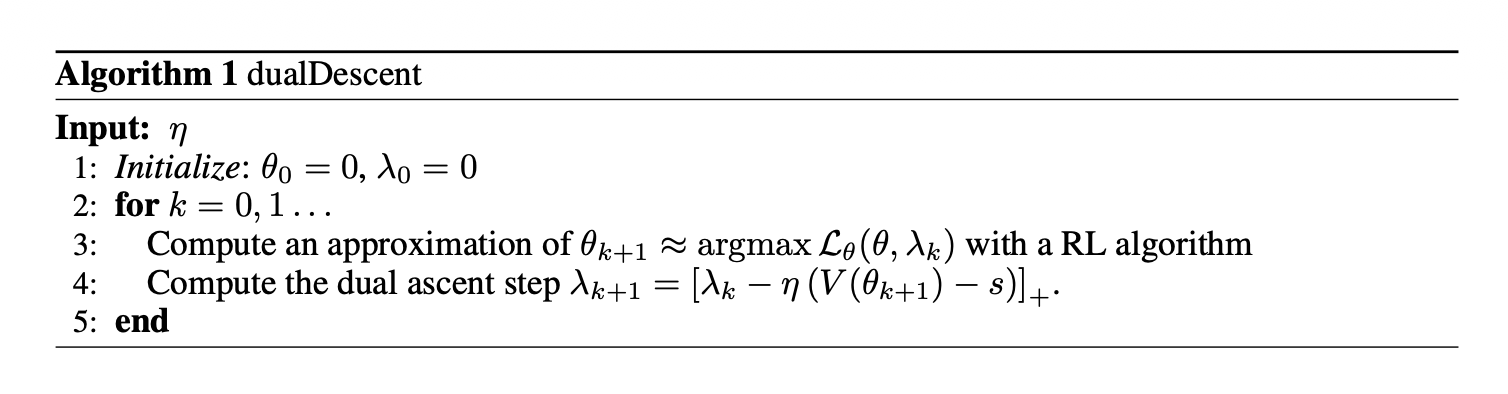
\includegraphics[width=1.0\linewidth]{figures/dualDescentAlgoPseudoCode.png}
            \label{fig:placeholder}
        \end{figure}

        \begin{remark}
        \begin{itemize}
            \item[$\bullet$] Line 3 could be itself a very slow subroutine.  
            \item[$\bullet$] According to last slides, a too poor parametrization could make the entire problem infeasible. ($D_\theta^* = -\infty, ~\lambda_\epsilon^*$ has infinite norm,...)
        \end{itemize}
        \end{remark}
    \end{frame}

\section{Instantaneous constrained problems (PI)}
    \begin{frame}{The "clipping" trick of (PI)}
        \vspace{-0.2cm}
        Let's move to problems with instantaneous constraints (PI): 
        \begin{align}
            \tag{PI}
            \max_{\pi} &~~ V_0(\pi) \triangleq \mathbb{E}_{s,\pi} \left[ \sum_{t=0}^{\infty} \gamma^t r_0(s_t, \pi(s_t)) \right]  \\
            \text{subject to } & ~\mathbb{E}_{\pi} \left[  r_i(s_t, \pi(s_t))  \right] \leq 0,~~  \forall t \in \{0,1,...\}, i \in \{1,2,...,m\}. \notag
        \end{align}

        Again, an extremely important assumption is: \textbf{Slater condition holds}. That is: (PI)'s feasible region has an nonempty relative interior. 

        Then a trick called "clipping" could be applied to (PI). Namely: if $r_i = \text{ReLU}(h_i)$ for some function $h_i$: 
        \begin{align*}
            & \mathbb{E}_{\pi} \left[ \text{ReLU} (h_i(s_t, \pi(s_t)))  \right] \leq 0 \iff \mathbb{E}_{\pi} \left[  r_i(s_t, \pi(s_t))  \right] \leq 0 \\ 
            \iff &  \mathbb{E}_{\pi} \left[ \sum_{t=0}^\infty \gamma^t \underbrace{\text{ReLU} (h_i(s_t, \pi(s_t)))}_{\text{treat as new constraints}} \right] \leq 0. 
        \end{align*} 

        Then, such (PI) can be cast to the previous (PC) framework... Emm, in fact, not really. The above may work, but could converge very slowly (\textcolor{teal}{later we see figures}).  
    \end{frame}

    \begin{frame}{A practical surrogate function}
        \vspace{-0.2cm}
        Inspired by augmented Lagrangian method (see e.g., Chapter 17 of \footnote{JS06 Numerical Optimization}), consider the following time-invariant instantaneous reward: 
        \begin{align}
            \tilde{r}(s_t,a_t) \triangleq r_0(s_t,a_t) - \sum_{i=1}^m \lambda_i \text{ReLU}(r_i(s_t,a_t)) - \frac{\rho}{2}\sum_{i=1}^m \text{ReLU}(r_i(s_t,a_t))^2. 
        \end{align}
        Denote $R(\pi, \lambda, \rho) \triangleq \mathbb{E}_{\pi} \left[ \sum_{t=0}^\infty \gamma^t \tilde{r}(s_t,\pi(s_t)) \right]$.
        
        Then, the algorithm is proposed as the following: 
        \begin{figure}
            \centering
            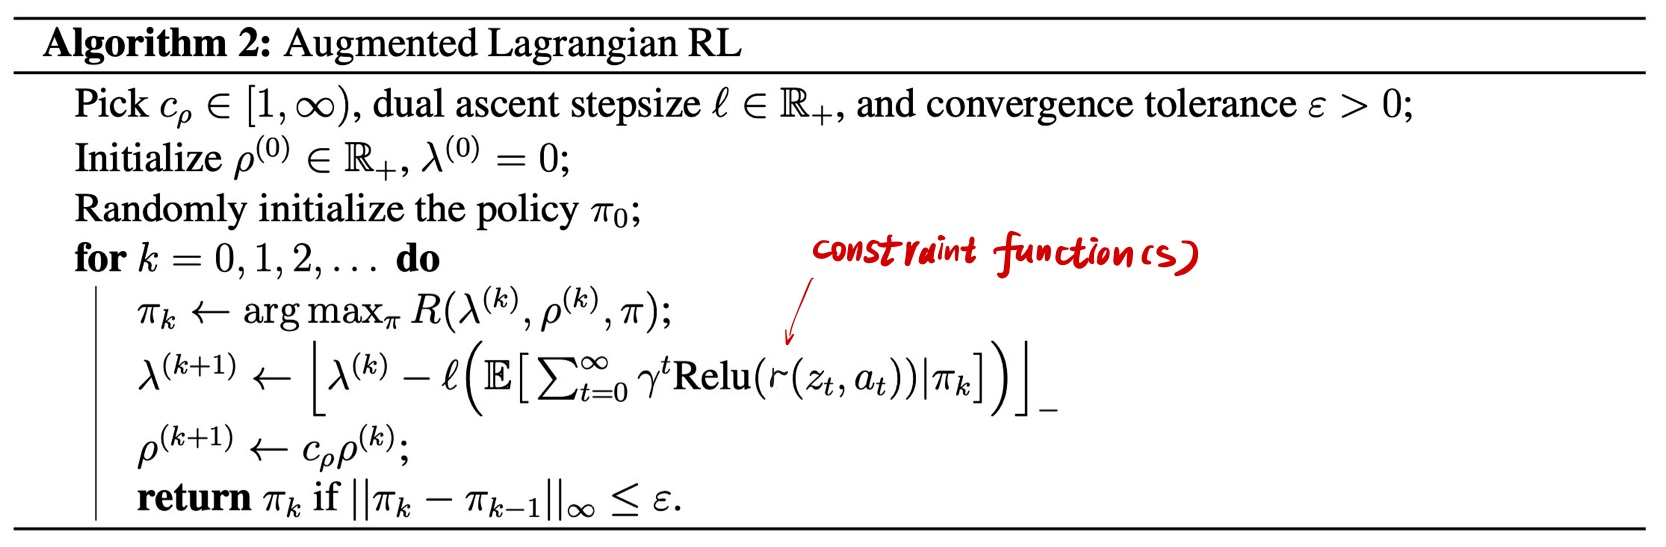
\includegraphics[width=0.9 \linewidth]{figures/ALM_algorithm.jpg}
            % \caption{Caption}
            \label{fig:placeholder}
        \end{figure}
    \end{frame}

    \begin{frame}{A detailed figure}
        \vspace{-0.5cm}
        \begin{figure}
            \centering
            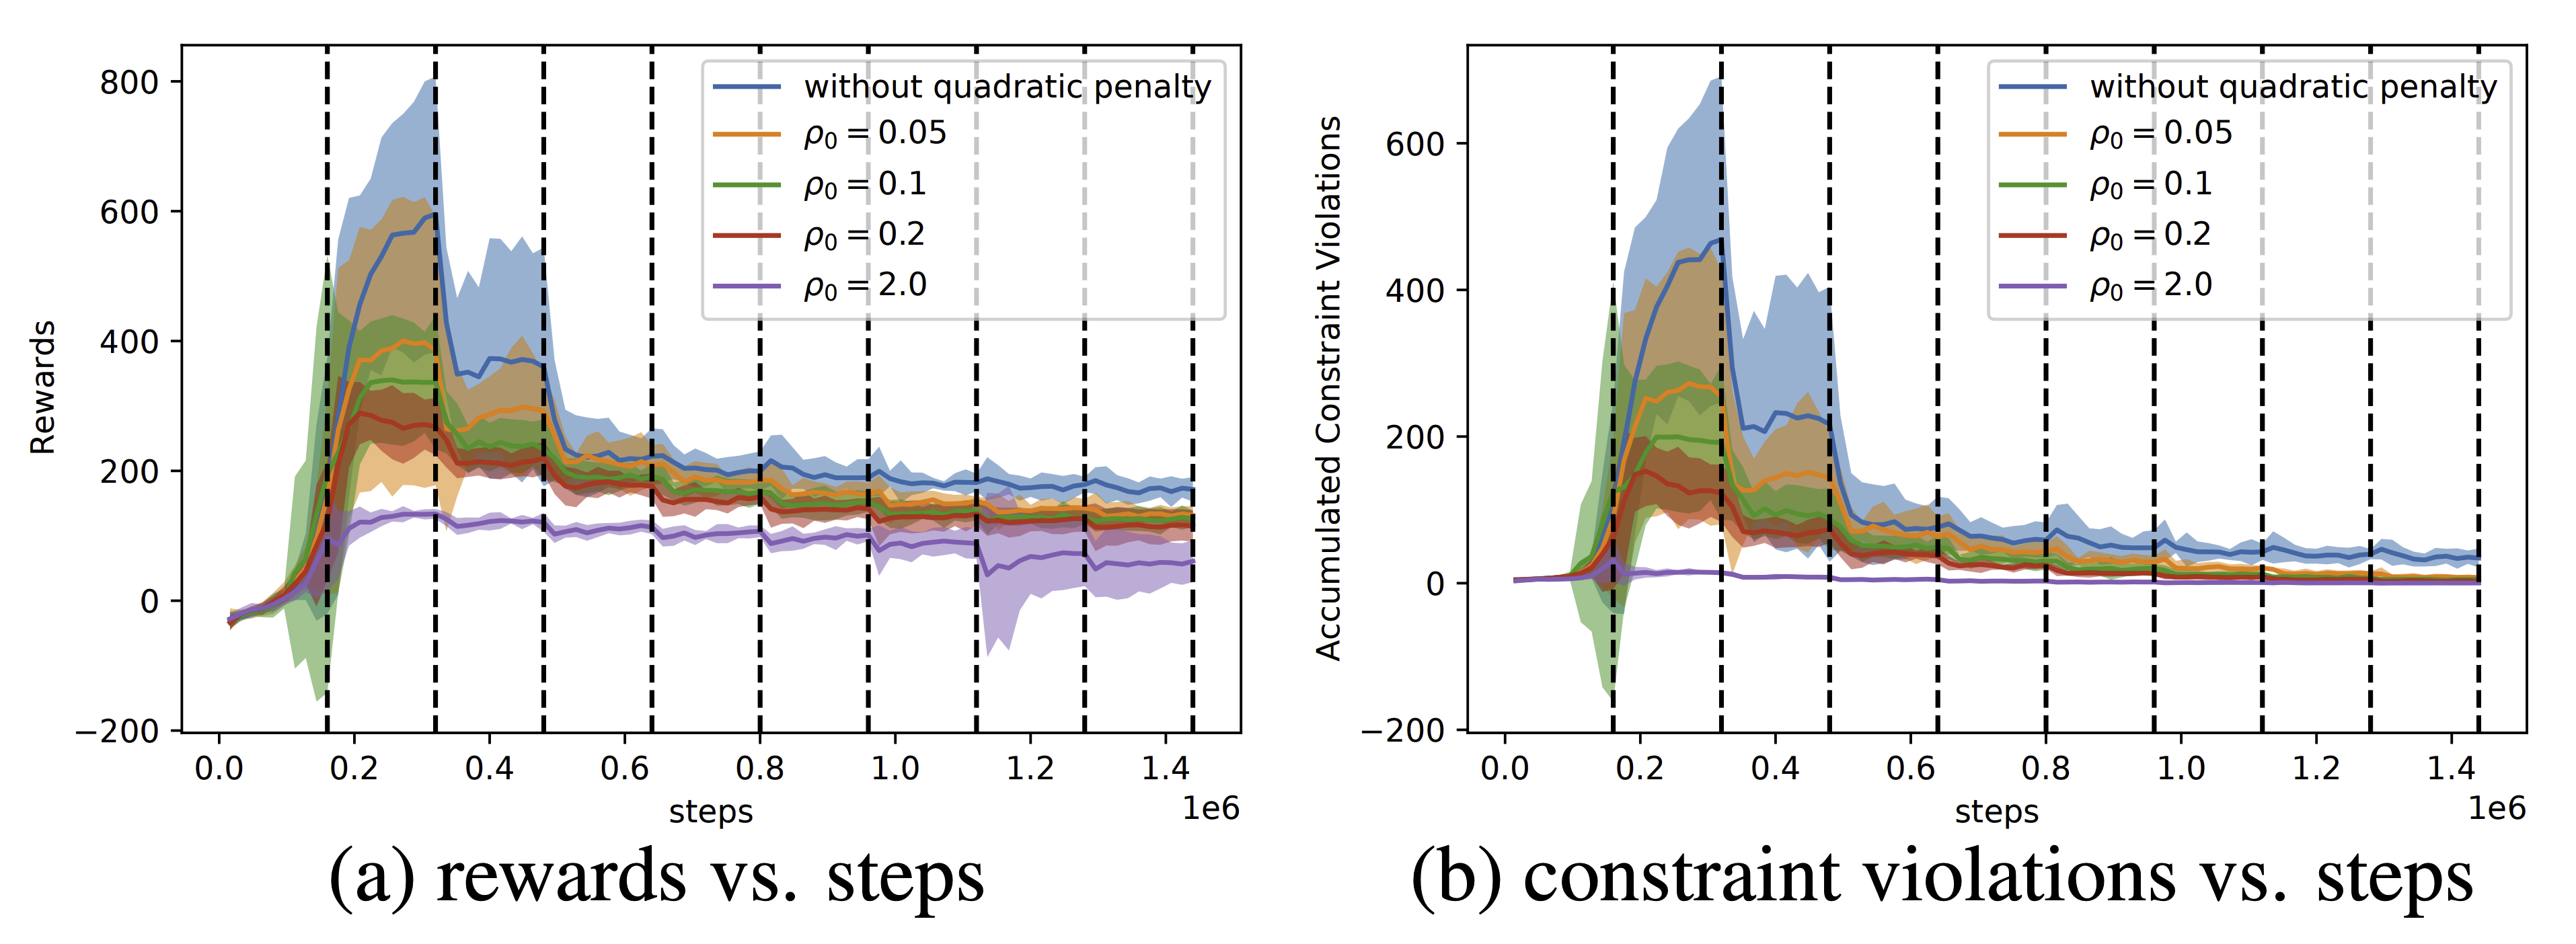
\includegraphics[width=1.01\linewidth]{figures/moving_bot_reward_violations.png}
            \label{fig:placeholder}
        \end{figure}

        \vspace{-0.4cm}
        \begin{block}{Some explanations}
        \begin{itemize}
            \item[$\bullet$] "Without quadratic" can gradually improve. But it seems to take more time.  
            \item[$\bullet$]  Increasing $\rho>0$ will let the agent to eliminate violations more quickly. But a larger $\rho$ will lead to possibly lower reward value (more conservative). 
        \end{itemize}
        \end{block}
    \end{frame}

    \begin{frame}{Some remarks}

        \vspace{-2cm}
        
        Rigorous instantaneous feasibility is hard to prove. Because there may be a policy $\pi_{in}$ being cumulatively feasible, and \textbf{instantaneously infeasible} (nearly feasible), meanwhile $\pi_{in}$ leads to a great reward. Then $\pi_{in}$ may be returned by the algorithm. 

        \vspace{0.3cm}
        If there exists a sequence $\{\pi_j\}_j$ of infeasible policy which instantaneous infeasibility of $\pi_j$ being $\frac{1}{j}$. Then there is no $\rho<\infty$ that can rule out all infeasible policies.

        \vspace{0.3cm}
        To eliminate such problem, further assumptions are needed. E.g., the problem is finite...
    \end{frame}


\begin{frame}
  \begin{center}
  {\fontsize{40}{50}\selectfont Thank You!}
  \end{center}
\end{frame}




%***************************************************************************
%***************************************************************************
\end{document}





































